\chapter{Metodologia}
\label{cap:metodologia}

Neste capítulo, descreve-se detalhadamente a metodologia experimental e computacional desenvolvida para a classificação preditiva de defeitos em rolamentos mecânicos. O fluxo de trabalho foi implementado integralmente em linguagem Python (versão 3.10+), utilizando as bibliotecas científicas de código aberto \textit{NumPy}, \textit{SciPy}, \textit{Pandas} e \textit{Scikit-Learn} \cite{pedregosa2011scikit, virtanen2020scipy}.

A arquitetura modular do pipeline de dados e modelagem é ilustrada na \autoref{fig:pipeline_metodologia}, estruturada em quatro macroetapas sequenciais: (i) Ingestão e Pré-processamento; (ii) Engenharia de Atributos; (iii) Particionamento e Validação Cruzada Agrupada; e (iv) Avaliação Preditiva Multiclasse e em Nível de Ensaio.

\begin{figure}[htbp]
    \centering
    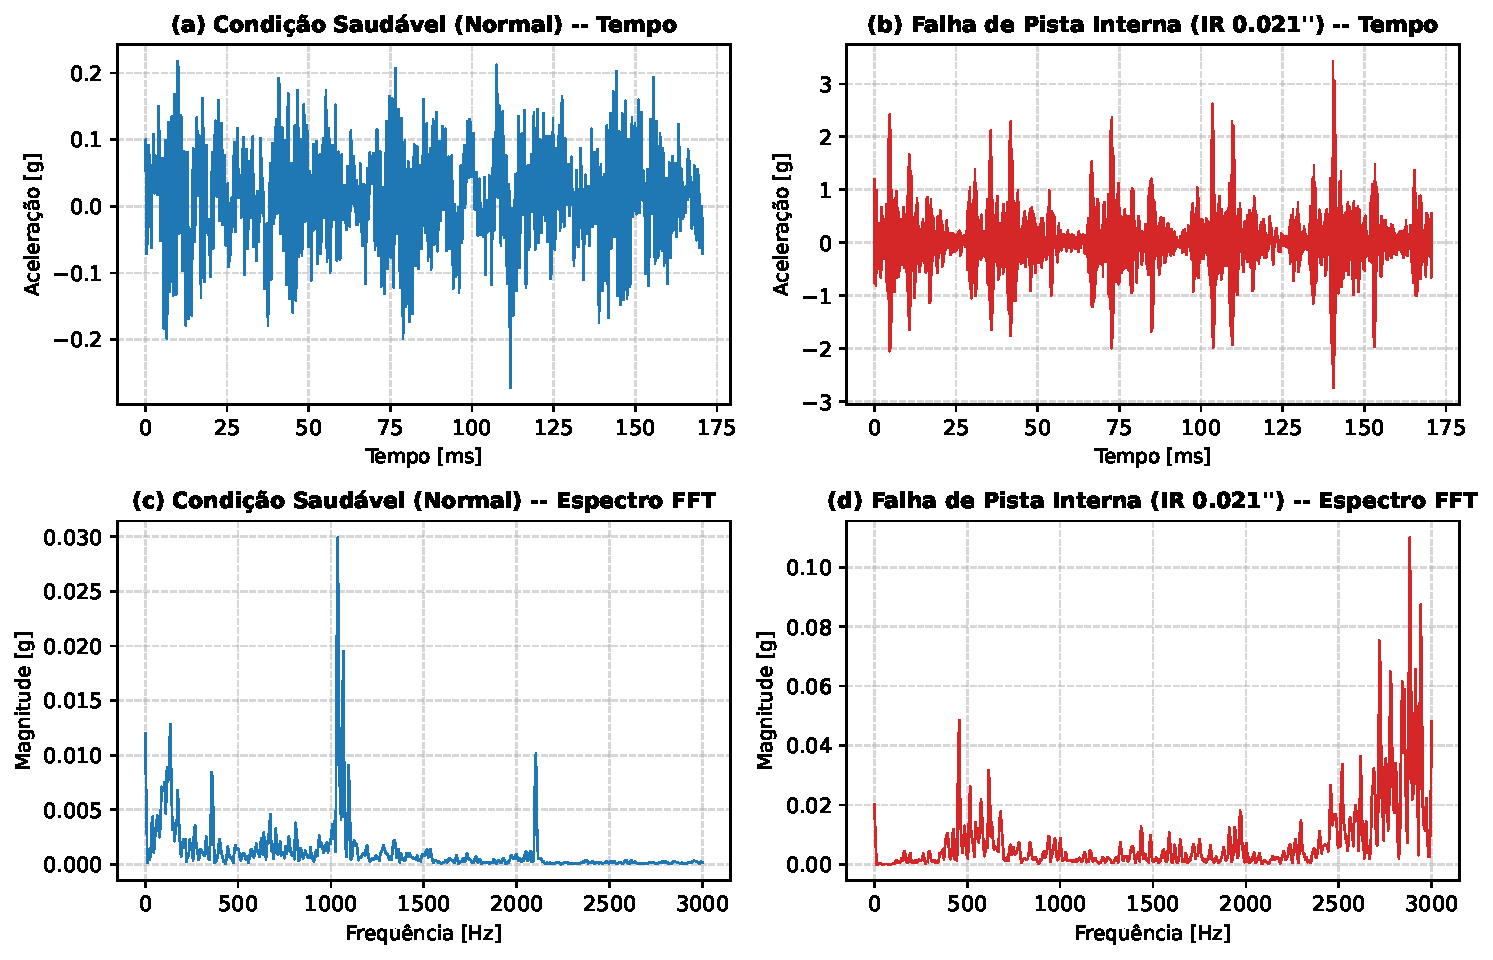
\includegraphics[width=0.95\textwidth]{fig_sinais_tempo_fft.pdf}
    \caption{Fluxograma metodológico do pipeline de engenharia de dados, extração de características e classificação de falhas}
    \label{fig:pipeline_metodologia}
    \legend{Fonte: Elaborado pelo autor (2026).}
\end{figure}

\section{Base de Dados Experimental (CWRU Bearing Dataset)}
\label{sec:dataset_cwru}

Para a validação científica dos modelos propostos, utilizou-se o banco de dados experimental do \textit{Bearing Data Center} da \textit{Case Western Reserve University} (CWRU), amplamente reconhecido na literatura internacional como o principal padrão de referência (\textit{benchmark}) para diagnóstico de mancais \cite{smith2015rolling}.

A bancada experimental da CWRU é constituída por um motor elétrico de indução trifásico de \SI{2}{\horsepower} (\SI{1,5}{\kilo\watt}), um transdutor de torque e encoder ótico acoplados a um eixo intermediário, e um dinamômetro de absorção de carga. O eixo é apoiado por dois mancais: um mancal na extremidade de acionamento (\textit{Drive End} -- DE), equipado com um rolamento de esferas de ranhura profunda SKF 6205-2RS JEM, e um mancal na extremidade oposta ao acionamento (\textit{Fan End} -- FE), com rolamento SKF 6203-2RS JEM. Neste trabalho, analisaram-se exclusivamente os sinais adquiridos pelo acelerômetro piezoelétrico acoplado magneticamente ao mancal \textit{Drive End} a uma frequência de amostragem de \SI{12}{\kilo\hertz} (\SI{12000}{amostras\per\second}).

Os parâmetros geométricos e operacionais do rolamento sob ensaio (SKF 6205-2RS JEM) são fundamentais para o cálculo analítico das frequências características de defeito e encontram-se sintetizados a seguir \cite{smith2015rolling}:
\begin{itemize}
    \item Diâmetro dos elementos rolantes (esferas): $d = \SI{0.3126}{in} \approx \SI{7,94}{\milli\meter}$;
    \item Diâmetro primitivo (\textit{pitch diameter}): $D = \SI{1.537}{in} \approx \SI{39,04}{\milli\meter}$;
    \item Número de esferas: $n = 9$;
    \item Ângulo de contato radial: $\phi = 0^\circ$ ($\cos\phi = 1,0$);
    \item Frequência de amostragem: $f_s = \SI{12000}{\hertz}$.
\end{itemize}

Os defeitos mecânicos foram induzidos artificialmente nos componentes do rolamento por meio de Usinagem por Descarga Elétrica (\textit{Electrical Discharge Machining} -- EDM / eletroerosão). Foram contempladas quatro condições de integridade física em três severidades de dano (\SI{0.007}{in}, \SI{0.014}{in} e \SI{0.021}{in}, equivalentes a \SI{0,18}{\milli\meter}, \SI{0,36}{\milli\meter} e \SI{0,53}{\milli\meter}) e quatro patamares de carregamento do motor (0, 1, 2 e \SI{3}{\horsepower}, resultando em velocidades angulares nominais de 1797, 1772, 1750 e \SI{1730}{rpm}).

A distribuição completa das classes, arquivos de ensaio e amostras geradas está apresentada na \autoref{tab:dataset_classes}.

\begin{table}[htbp]
    \centering
    \caption{Estrutura de classes, severidades e distribuição de amostras do dataset CWRU (12 kHz)}
    \label{tab:dataset_classes}
    \begin{tabular}{lllcc}
        \toprule
        \textbf{Classe} & \textbf{Descrição Física} & \textbf{Severidades (Diâmetro)} & \textbf{Ensaios} & \textbf{Janelas ($N=2048$)} \\
        \midrule
        \textbf{B} & Elemento Rolante & \SI{0.007}{in}, \SI{0.014}{in}, \SI{0.021}{in} & \num{12} & \num{708} \\
        \textbf{IR} & Pista Interna & \SI{0.007}{in}, \SI{0.014}{in}, \SI{0.021}{in} & \num{12} & \num{709} \\
        \textbf{Normal} & Condição Saudável & N/A & \num{4} & \num{828} \\
        \textbf{OR} & Pista Externa (@6:00) & \SI{0.007}{in}, \SI{0.014}{in}, \SI{0.021}{in} & \num{12} & \num{708} \\
        \midrule
        \textbf{Total} & \textbf{4 Condições Físicas} & \textbf{3 Níveis + Baseline} & \textbf{\num{40}} & \textbf{\num{2953}} \\
        \bottomrule
    \end{tabular}
    \legend{Fonte: Elaborado pelo autor com base nos dados da Case Western Reserve University (2026).}
\end{table}


\section{Pré-processamento e Segmentação por Janelas Deslizantes}
\label{sec:segmentacao}

Os arquivos brutos em formato binário do MATLAB (\texttt{.mat}) foram processados pelo módulo \texttt{src/preprocessing.py}. O sinal de aceleração contínuo de cada ensaio apresenta durações que variam entre \num{121000} amostras (\SI{10}{\second}) e \num{485000} amostras (\SI{40}{\second}).

\subsection{Segmentação Temporal (Sliding Window)}
Para converter cada série temporal contínua em instâncias discretas adequadas para aprendizado supervisionado, aplicou-se a técnica de segmentação por janelas deslizantes (\textit{sliding window}). O sinal discretizado de um ensaio $x[n]$ é particionado em $M$ janelas discretas de comprimento fixo $N$:
\begin{equation}
    \mathbf{w}_m = [x[m \cdot S], x[m \cdot S + 1], \dots, x[m \cdot S + N - 1]]^T, \quad m = 0, 1, \dots, M-1
    \label{eq:sliding_window}
\end{equation}
onde:
\begin{itemize}
    \item $\mathbf{w}_m$ é o vetor de $N$ pontos correspondente à $m$-ésima janela;
    \item $N$ é o comprimento da janela temporal (adotou-se $N = 2048$ pontos);
    \item $S$ é o passo de deslocamento da janela (\textit{stride});
    \item O fator de sobreposição (\textit{overlap}) é definido por $O = 1 - S/N$. No pipeline de validação base deste trabalho, adotou-se janelamento contíguo sem sobreposição ($O = 0$, $S = N = 2048$), gerando amostras estatisticamente independentes no domínio do tempo.
\end{itemize}

A escolha de $N = 2048$ pontos a uma taxa de amostragem $f_s = \SI{12}{\kilo\hertz}$ estabelece uma duração temporal de janela de:
\begin{equation}
    \Delta t = \frac{N}{f_s} = \frac{2048}{12000} \approx \SI{0,1707}{\second}
    \label{eq:duracao_janela}
\end{equation}

Considerando a rotação média do eixo sob carga ($f_r \approx \SI{29,5}{\hertz}$, equivalente a \SI{1772}{rpm}), o período fundamental de uma rotação do eixo é de $T_{\text{rot}} = 1/f_r \approx \SI{0,0339}{\second}$. Dessa forma, cada janela de $2048$ pontos abrange aproximadamente:
\begin{equation}
    N_{\text{rot}} = \frac{\Delta t}{T_{\text{rot}}} \approx \frac{0,1707}{0,0339} \approx 5,03 \text{ rotações completas do eixo}
    \label{eq:num_rotacoes}
\end{equation}

Esse intervalo garante a quase-estacionariedade do sinal de vibração e assegura resolução temporal e em frequência suficientes ($\Delta f = f_s / N = 12000 / 2048 \approx \SI{5,86}{\hertz}$) para capturar com precisão as manifestações impulsivas dos defeitos.

\subsection{Rastreabilidade Temporal e Tratamento de Metadados}
Diferentemente de pipelines convencionais que descartam a procedência das amostras, implementou-se uma estrutura de linhagem de dados (\textit{data lineage}) no DataFrame gerado. Cada linha armazena:
\begin{itemize}
    \item Identificador do arquivo físico de origem (\texttt{arquivo});
    \item Índice sequencial da janela (\texttt{janela\_idx});
    \item Amostras de início e fim no sinal contínuo original (\texttt{sample\_start} e \texttt{sample\_end});
    \item Rótulo de condição física (\texttt{classe}: Normal, IR, B, OR);
    \item Severidade do dano mecânico e nível de carga do motor elétrico.
\end{itemize}

Nos arquivos de condição saudável sob carga de 1 e \SI{2}{\horsepower} (\texttt{Normal\_1.mat} e \texttt{Normal\_2.mat}), a velocidade angular ($\text{RPM}$) não foi registrada originalmente no arquivo MAT da CWRU. Para manter a consistência física dos cálculos cinemáticos espectrais, aplicou-se a imputação automática através da mediana de rotação dos demais ensaios operando sob a mesma condição de carga do motor (\texttt{preencher\_rpm\_ausente}).

\section{Engenharia e Extração de Atributos}
\label{sec:extracao_features}

Para cada janela discreta de sinal $\mathbf{w}_m \in \mathbb{R}^{2048}$, o módulo \texttt{src/features.py} computa um vetor estruturado de características multidimensional $\mathbf{x}_m \in \mathbb{R}^{16}$, composto por 8 atributos estocásticos no domínio do tempo e 8 atributos espectrais no domínio da frequência:

\begin{enumerate}
    \item \textbf{Atributos no Domínio do Tempo (8 descritores):}
    \begin{itemize}
        \item Valor Eficaz ($\text{RMS}$), via \autoref{eq:rms};
        \item Curtose ($K$), via \autoref{eq:curtose} (referência em 3,0 com \texttt{fisher=False});
        \item Fator de Crista ($\text{CF}$), via \autoref{eq:fator_crista};
        \item Desvio Padrão ($\sigma$), via \autoref{eq:desvio_padrao};
        \item Coeficiente de Assimetria ($S$), via \autoref{eq:assimetria};
        \item Amplitude Pico a Pico ($X_{p-p}$), via \autoref{eq:pico_a_pico};
        \item Fator de Forma ($\text{SF}$) e Fator de Impulso ($\text{IF}$), via \autoref{eq:fatores_forma_impulso}.
    \end{itemize}
    \item \textbf{Atributos no Domínio da Frequência e Análise de Envelope (8 descritores):}
    \begin{itemize}
        \item Energias Espectrais em torno de BPFO, BPFI, BSF e FTF: o sinal da janela é submetido à Transformada de Hilbert para extração do envelope de amplitude instantânea, com remoção do componente médio DC (\autoref{eq:envelope_sem_dc}). Em seguida, calcula-se a FFT do envelope ponderada por janela de Hanning. A energia de cada frequência de falha é quantificada pela magnitude máxima na banda centrada em $\pm \SI{5,0}{\hertz}$ em torno da frequência teórica calculada via \autoref{eq:bpfo} a \ref{eq:ftf};
        \item Centroide Espectral: centro de gravidade da distribuição de frequência no espectro direto da FFT;
        \item Variância Espectral: dispersão da energia em torno do centroide espectral;
        \item Frequência de Pico Dominante e Amplitude de Pico Dominante no espectro da FFT direta.
    \end{itemize}
\end{enumerate}

\subsection{Contratos de Dados e Persistência}
Antes da etapa de treinamento dos modelos, o conjunto de dados processado é submetido a testes automatizados de qualidade de dados (\textit{data quality contracts}), implementados na rotina \texttt{validar\_qualidade\_features}. Os testes verificam a ausência estrita de valores nulos (\textit{missing values}) e infinitos gerados por divisões numéricas, e validam limites de domínio físico ($\text{RMS} \ge 0$, $\text{CF} \ge 1,0$).

A base tratada é então persistida no formato colunar de alto desempenho Apache Parquet (\texttt{data/processed/features.parquet}), o qual preserva os tipos de dados originais de cada coluna e acelera as rotinas analíticas subsequentes, mantendo-se concomitantemente uma cópia em formato CSV.

\section{Protocolo de Treinamento e Prevenção de Data Leakage}
\label{sec:protocolo_treinamento}

\subsection{Prevenção Crítica de Vazamento de Dados (Data Leakage)}
Em problemas de análise de vibração em máquinas rotativas, a divisão ingênua de janelas temporais de forma aleatória (\textit{random train-test split}) constitui uma falha metodológica severa comum na literatura. Como janelas vizinhas de um mesmo ensaio compartilham condições operacionais idênticas, desgaste idêntico e transientes altamente correlacionados, misturar janelas do mesmo ensaio nos conjuntos de treino e teste induz a um vazamento de dados (\textit{data leakage}). Esse fenômeno produz métricas de acurácia artificialmente infladas no laboratório, mas que falham drasticamente quando o modelo é confrontado com uma máquina ou rolamento nunca antes visto \cite{smith2015rolling}.

Neste trabalho, garantiu-se a estrita integridade metodológica adotando-se o princípio da \textbf{partição em nível de arquivo de ensaio}:
\begin{enumerate}
    \item \textbf{Divisão Treino/Teste Independente (70\% / 30\%):} O particionamento estratificado é aplicado sobre a lista de arquivos físicos de ensaio (\texttt{arquivo}), de modo que todos os \num{2048} pontos e todas as janelas pertencentes a um arquivo de teste específico jamais sejam apresentados ao modelo durante o treinamento. Dos 40 ensaios originais, 28 arquivos (\num{2067} janelas) integraram o conjunto de treino e 12 arquivos (\num{886} janelas) compuseram o conjunto de teste independente;
    \item \textbf{Validação Cruzada Estratificada Agrupada (\textit{Stratified Group K-Fold}):} Para a otimização de hiperparâmetros e estimativa de generalização, implementou-se uma validação cruzada com $k = 4$ dobras (\textit{folds}). As amostras foram agrupadas pela coluna \texttt{arquivo} e estratificadas pela \texttt{classe}, assegurando que nenhuma dobra de teste contenha janelas de arquivos presentes na dobra de treino correspondente.
\end{enumerate}

\subsection{Padronização de Escala (Feature Scaling)}
Como os atributos extraídos apresentam ordens de grandeza distintas (por exemplo, valores de RMS em torno de \SI{0.1}{g} e energias espectrais superiores a \num{20}), aplicou-se a padronização por pontuação-z (\textit{StandardScaler}) para os modelos sensíveis à distância euclidiana, como o SVM:
\begin{equation}
    \tilde{x}_{ij} = \frac{x_{ij} - \mu_j}{\sigma_j}
    \label{eq:standard_scaler}
\end{equation}
onde $\mu_j$ e $\sigma_j$ são a média e o desvio padrão da $j$-ésima característica calculados \textbf{exclusivamente sobre o conjunto de treinamento}, sendo posteriormente aplicados para transformar o conjunto de teste, prevenindo vazamento de parâmetros de escala.

\subsection{Configuração e Otimização dos Classificadores}
Os modelos \textit{Random Forest} e \textit{Support Vector Machines} foram implementados conforme as especificações detalhadas na \autoref{tab:hiperparametros}, utilizando pipelines encapsulados do \textit{Scikit-Learn} que integram pré-processamento e estimação preditiva.

\begin{table}[htbp]
    \centering
    \caption{Espaço de busca da validação cruzada e hiperparâmetros finais dos modelos}
    \label{tab:hiperparametros}
    \begin{tabular}{lll}
        \toprule
        \textbf{Classificador} & \textbf{Espaço de Otimização (Grid Search)} & \textbf{Configuração Adotada} \\
        \midrule
        \multirow{4}{*}{\textbf{Random Forest}} 
        & Número de Árvores (\textit{n\_estimators}): $[50, 100, 200]$ & \textit{n\_estimators} = \num{100} \\
        & Critério de Divisão (\textit{criterion}): $[\text{Gini}, \text{Entropia}]$ & \textit{criterion} = Gini \\
        & Profundidade Máxima (\textit{max\_depth}): $[\text{None}, 10, 20]$ & \textit{max\_depth} = None \\
        & Amostras Mínimas por Divisão: $[2, 5, 10]$ & \textit{min\_samples\_split} = \num{2} \\
        \midrule
        \multirow{4}{*}{\textbf{SVM}} 
        & Pré-processamento: $[\text{StandardScaler}, \text{MinMaxScaler}]$ & Padronização (\textit{StandardScaler}) \\
        & Função de \textit{Kernel}: $[\text{Linear}, \text{RBF}, \text{Polinomial}]$ & \textit{Kernel} Radial Base (RBF) \\
        & Parâmetro de Regularização ($C$): $[0.1, 1.0, 10.0, 100.0]$ & $C = 1.0$ \\
        & Coeficiente do \textit{Kernel} ($\gamma$): $[\text{scale}, \text{auto}, 0.01, 0.1]$ & $\gamma = \text{scale} \approx 0.0625$ \\
        \bottomrule
    \end{tabular}
    \legend{Fonte: Elaborado pelo autor (2026).}
\end{table}


\subsection{Estratégia de Votação Majoritária por Ensaio (File-Level Voting)}
Em uma aplicação ferroviária embarcada real, o objetivo primário consiste em diagnosticar o estado do mancal físico como um todo, e não emitir alarmes isolados baseados em uma única janela de \SI{0,17}{\second}. Para mitigar ruídos espúrios passageiros, desenvolveu-se uma rotina de votação majoritária agregada por ensaio (\textit{file-level majority voting}):
\begin{equation}
    \hat{C}_{\text{ensaio}} = \text{Moda} \left\{ \hat{y}_1, \hat{y}_2, \dots, \hat{y}_{M_{\text{ensaio}}} \right\}
    \label{eq:file_voting}
\end{equation}
onde $\hat{y}_m$ é a classe predita pelo modelo supervisionado para a $m$-ésima janela do arquivo sob análise.
